\chapter{Equazioni non lineari}

\section{Metodo di bisezione}
Deriva dal teorema degli zeri per funzioni continue:
\quote{Se $f(x)$ è continua su $[a,b]$ e $f(a)f(b)<0$ allora esiste almeno un $x\in[a,b]$ tale che $f(x)=0$.}

Posso creare un semplice algoritmo che prende il punto media dell'intervallo di modo da 
ottenere il punto $c=\frac{a+b}{2}$.

Se $c=0$ allora ho trovato una radice, se non e' uguale a zero bisogna guardare l'intervallo
dove la $f(x)$ cambia di segno.

Si continua con queste iterazioni fino ad ottenere una radice.

\begin{figure}[h!]
  \centering
  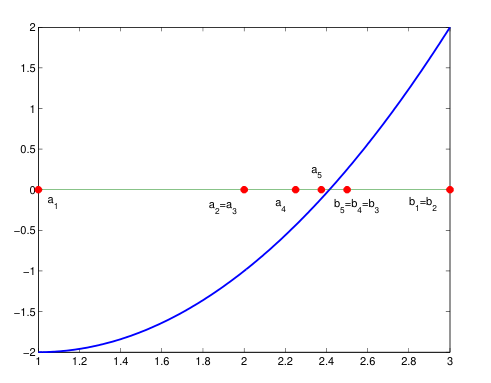
\includegraphics[width=0.5\linewidth]{./images/bisezione.png}
  \label{fig:bisezione}
  \caption{Esempio di metodo di bisezione}
\end{figure}

Il metodo di bisezione ha un ordine di convergenza lineare.

Se vogliamo fissare una tolleranza $\varepsilon$ e otteniamo:
\begin{equation}
  k \geq \frac{\log_{10}(\frac{b-a}{\varepsilon})}{\log_{10}2} \approx 3.32192 \log_{10}\frac{b-a}{\varepsilon}
\end{equation}


In media e' necessario 3.3 bisezioni per migliorare di una cifra significativa l'accuratezza della radice.

Bisogna quindi sfruttare altri metodi per velocizzare la discesa verso la radice come derivate.

\section{Metodo delle secanti}
\begin{figure}[h!]
  \centering
  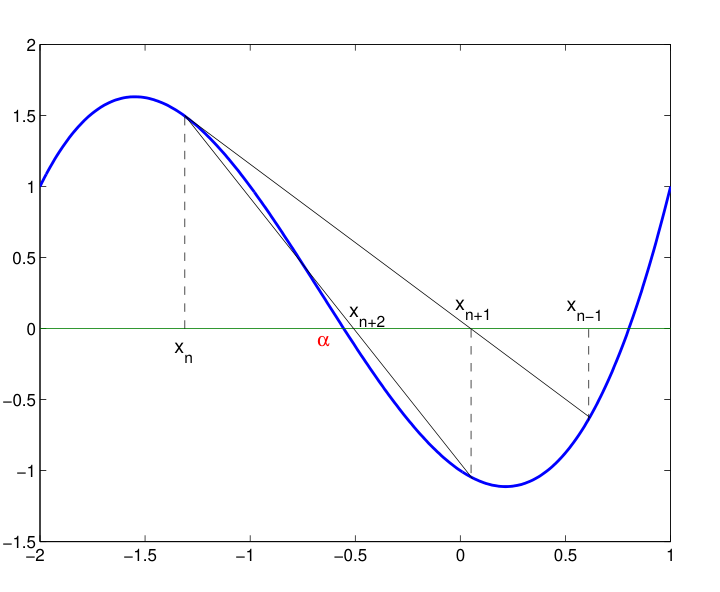
\includegraphics[width=0.5\linewidth]{./images/secanti.png}
  \label{fig:secanti}
  \caption{Esempio di metodo delle secanti}
\end{figure}
Con il metodo delle secanti si costruisce una successione di punti ${x_k}$ tali che:
\quote{
Per ogni $k \geq 1$ il putno $x_{k+1}$ e' lo zero della retta secante che passa per i punti

}
\begin{equation} 
  (x_{k-1}, f(x_{k-1})), \quad (x_k, f(x_k))
\end{equation}

Quindi otteniamo un sistema:
\begin{equation}
  \begin{cases}
    y = 0 \\
    y = \frac{f(x_k)-f(x_{k-1})}{x_k-x_{k-1}} x + \frac{f(x_{k-1})x_k-f(x_k)x_{k-1}}{x_k-x_{k-1}}
  \end{cases}
\end{equation}

Dal sistema otteniamo la forma del metodo delle secanti, che pero' richiede due punti iniziali
$x_0$ e $x_1$:
\begin{equation}
  x_{k+1} = x_k - f(x_k)\frac{x_k-x_{k-1}}{f(x_k)-f(x_{k-1})} \quad k\geq 1
\end{equation}

Se la funzione $f(x)$ e' convessa o concava nell'intervallo $[a, b]$, la succession
${x_k}$ converge ad $\alpha$ in modo monotono, crescente oppure decrescente.

Percio' posso controllare l'approssimazione del risultato mediante la distanza tra $x_{n+1}$ 
e $x_n$ con il criterio di arresto:
\begin{equation}
  |x_{n+1}-x_n| < \varepsilon
\end{equation}

Dove $\varepsilon > 0$ e' la tolleranza prefissata.

% Se la funzione ha una continuita' di ordine 1 ($f \in C_1([a, b])$) grazie alal formula di Taylor
% si ha che $f(x_n) = (x_n - \alpha)f'(\epsilon)$

\section{Metodo delle tangenti}
\begin{figure}[h!]
  \centering
  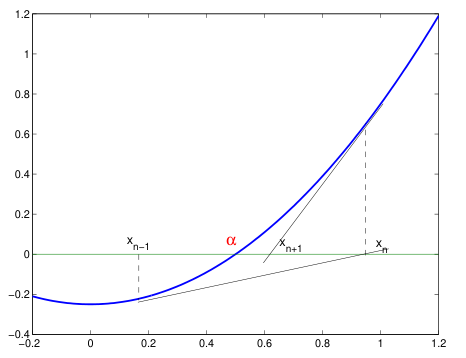
\includegraphics[width=0.5\linewidth]{./images/tangenti.png}
  \label{fig:tangenti}
  \caption{Esempio di metodo delle tangenti}
\end{figure}
Sotto certe ipotesi performa meglio dei due mtodi di prima, ma si applica solo se la funzione
e' derivabile ndell'intervallo.

Si procede con:
\begin{itemize}
  \item Si sceglie un punto $x_0$ dell'intervallo $[a, b]$ \textbf{opportuno}
  \item si considera la retta tangente nel punto $(x_0, f(x_0))$ di equazione $y = f(x_0) + f'(x_0)(x-x_0)$
  \item Il punto $x_1$ interseca l'asse delle $x$ ($y=0$)
\end{itemize}

\begin{equation}
  x_1 = x_0 - \frac{f(x_0)}{f'(x_0)}
\end{equation}

Se il punto $x_0$ e' stato scelto correttamente, il punto $x_1$ cade nell'intervallo $[a, b]$
e risulta compreso tra $\alpha$ e $x_0$.

\begin{itemize}
  \item si sostituisce il punto $x_0$ con il nuovo punto $x_1$
  \item si calcola il prossimo punto $x_2$
\end{itemize}

Dato un punto $x_0$ si itera la formula per ottenere tutti gli altri punti:
\begin{equation}
  x_{n+1} = x_n - \frac{f(x_n)}{f'(x_n)}, \quad i = 0, 1, \dots
\end{equation}

Ogni iterazione di qursto metodo richiede la valutazione della funzione e della sua derivata.


Nel caso la funzione sia derivabile 2 volte, si puo' usare il seguente teorema:
\quote{
Sia $f(x) \in C^2([a, b])$ e $f'(x) \neq 0$, $f''(x) \neq 0\quad \forall x \in [a, b]$,
escluso al piu' il punto $\alpha$.
Se (esiste) un punto $x_0 \in [a, b]$ tale che $f(x_0)f''(x_0) > 0$ allora la successione generata dal 
metodo delle tangenti e' monotona convergente alal radice $\alpha$.
}

\section{Metodi iterativi}
La funzione $g(x)$ e' detta funzione di iterazione e le sue soluzioni sono detti punti fissi
di $g(x)$.

Per semplicita' considero $g\in C^1[a, b]$
